% RA-L submission. Build: latexmk -pdf paper.tex   (live: latexmk -pdf -pvc paper.tex)
% Limit: 6 pages included, up to 8 with overlength fee, references included. Check the current RA-L author guidelines.
\documentclass[letterpaper, journal, twoside]{IEEEtran}

\usepackage{amsmath,amssymb}
\usepackage{graphicx}
\usepackage{booktabs}
\usepackage{multirow}
\usepackage{url}
\usepackage{algorithm}
\usepackage{algpseudocode}
\usepackage[dvipsnames]{xcolor}
\usepackage{tikz}
\usetikzlibrary{arrows.meta,calc,shapes.geometric}
\DeclareRobustCommand{\todo}[1]{\textcolor{red}{[TODO: #1]}}  % robust: the title and headers uppercase their text
\newcommand{\figplaceholder}[2]{\fbox{\parbox[c][#2][c]{0.95\linewidth}{\centering\textcolor{red}{#1}}}}

\begin{document}

\title{Reconfiguration-Aware Co-Optimization of Object Placement and Coverage Path for Robot Arms}

\author{Zhenwei Liu%
\thanks{\todo{Affiliations, funding.}}}


\maketitle

\begin{abstract}
In many industrial robot applications, such as surface inspection, spraying, and cleaning, a fixed-base robot arm must traverse a set of viewpoints pre-generated from an object's surface geometry. This requires selecting the object placement, the visiting order, and an inverse kinematics (IK) solution for each viewpoint. A suboptimal placement leaves viewpoints unreachable and forces reconfigurations, where the robot arm must switch joint configurations between consecutive viewpoints. Existing methods optimize the placement and the coverage path separately or without explicitly reducing reconfigurations. We propose a kinematics-based method that jointly optimizes the object position and the coverage path while explicitly reducing reconfigurations. We unify viewpoint reach and reconfiguration reduction by treating a viewpoint as missed if it is unreachable or requires a reconfiguration, based on the key observation that both occur when a kinematic margin of joint limits, singularities, or collisions shrinks to zero. The method alternates between two modules. Kinematic margin expansion (KME) moves the object along a gradient that increases the kinematic margins at missed viewpoints, so that more viewpoints are reached and reconfigurations are reduced. Coverage-path placement descent (CPD) moves the object to shorten the coverage path, while the visiting order and IK solutions are re-solved as a generalized traveling salesman problem. In simulation, the method achieves a high success rate and yields 8--30\% shorter paths and 34--49\% fewer reconfigurations than baselines. We further validate the method on a real UR3e robot arm.
\end{abstract}

\begin{IEEEkeywords}
Motion and Path Planning; Industrial Robots; Manipulation Planning; Task Planning.
\end{IEEEkeywords}

\section{Introduction}
\IEEEPARstart{M}{any} industrial robot applications, such as surface inspection, 3D reconstruction, painting, and cleaning, require a fixed-base robot arm to traverse the surface of an object, with a camera or a nozzle attached to its end-effector. In those applications, a set of viewpoints is typically pre-generated based on the object's surface geometry~\cite{tang2024viewpoint,do2023depowdering}. The object is then placed in the workcell, and the robot arm follows a coverage path that visits every viewpoint once to perform the task. The quality of the coverage path, however, depends critically on the object placement. For example, a suboptimal placement may leave viewpoints unreachable due to joint limits, singularities, or collisions. It may also yield an inefficient coverage path with frequent reconfigurations, where the robot arm must deviate from the current path, switch its joint configuration, and then resume task execution. A reconfiguration is costly: the large joint sweep adds cycle time and collision risk, and the discontinuous end-effector motion interrupts continuous processes such as painting or scanning.
\begin{figure}[!t]
\centering
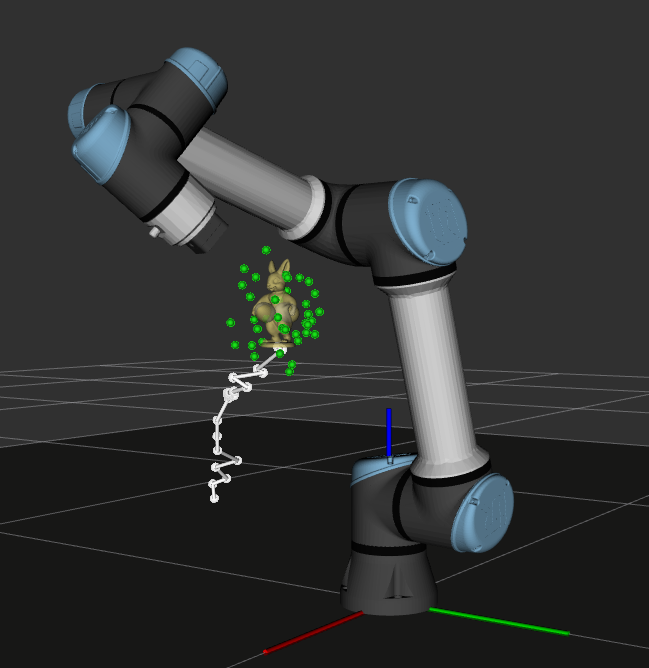
\includegraphics[width=0.7\linewidth]{figures/teaser.png}
\caption{A UR5e inspecting an object from given viewpoints (green). Starting below the robot arm, the object is moved (white trail) to a placement where every viewpoint is reachable with a short coverage path and few reconfigurations. \todo{Replace with the Stanford bunny or Armadillo, white background; ideally baseline vs.\ ours from the same start.}}
\label{fig:teaser}
\end{figure}

Some works place the object empirically and drop the unreachable viewpoints~\cite{do2023depowdering}, which requires trial and error and sacrifices coverage. Other methods use precomputed reachability or inverse reachability maps~\cite{zacharias2007capturing,vahrenkamp2013robot}. However, their accuracy relies heavily on the sampling density of the robot's workspace and may compromise computational efficiency during planning. Moreover, these maps evaluate each viewpoint independently and thus ignore the path between consecutive viewpoints. Other works avoid such maps by optimizing the placement directly. Mayer and Althoff~\cite{mayer2026smart} use stochastic gradient descent (SGD) to move the robot base until every viewpoint is reachable, but ignore the path cost. Sampling-based and derivative-free methods~\cite{spensieri2016,baizid2015,wachter2024placement} can include the path cost, but treat it as a black box and need many evaluations. B*~\cite{bstar2025} jointly optimizes the base position and the joint configurations, but assumes a fixed visiting order and no reconfigurations. Conversely, task-sequencing methods~\cite{alatartsev2015survey,suarezruiz2017robotsp} optimize the order and IK solutions as a generalized traveling salesman problem (GTSP), but take the placement as given.

In this paper, we propose a method that jointly optimizes the object position and the coverage path while explicitly reducing the number of reconfigurations, without requiring a predefined visiting order. We unify viewpoint reach and reconfiguration reduction by treating a viewpoint as missed when it is either unreachable or requires a reconfiguration from the previous viewpoint. Both problems are addressed by \emph{kinematic margin expansion} (KME), where the \emph{kinematic margins} measure how far the robot arm is from joint limits, singularities, and collisions. KME moves the object along a gradient that increases these kinematic margins at missed viewpoints while preserving, where possible, the margins at reached viewpoints. This unification rests on our key observation that unreachable viewpoints and reconfigurations share the same cause: a kinematic margin shrinks to zero. A viewpoint is unreachable when the robot arm runs out of kinematic margin during the reach, and a reconfiguration occurs when the robot arm runs out of kinematic margin while moving between two consecutive viewpoints. These margins are locally differentiable with respect to the object position, and their gradients are obtained through the robot Jacobian. In addition, we propose \emph{coverage-path placement descent} (CPD), which moves the object along the gradient of the path cost while re-solving the visiting order and IK solutions at every object position as a GTSP that penalizes reconfigurations. Unlike staged methods that first find a reachable placement and then plan the coverage path at it, our method resolves reach, reconfigurations, and the coverage path in a single optimization loop: the GTSP plans through every viewpoint from the first iteration, including the missed ones through their closest IK, so the path is shortened while viewpoints are still being reached.

Our contributions are:
\begin{itemize}
  \item A unified formulation of viewpoint reach and reconfiguration reduction, which treats a viewpoint as missed when it is either unreachable or requires a reconfiguration, solved by \emph{kinematic margin expansion} (KME): a kinematics-based object motion that expands the joint-limit, singularity, and collision kinematic margins for missed viewpoints so that more viewpoints can be reached and reconfigurations are reduced.
  \item Coverage-path placement descent (CPD): the object moves along the gradient of the path cost, while the visiting order and IK solutions are re-solved at every object position as a GTSP that penalizes reconfigurations, rather than only at a fixed placement. Since the GTSP also plans through missed viewpoints, reach, reconfigurations, and the coverage path are resolved in a single descent rather than in stages.
  \item An evaluation on a 7-DOF and a 6-DOF robot arm from 32 initial object placements each, against SGD~\cite{mayer2026smart} and CMA-ES~\cite{hansen2016cmaes} placement that use the same GTSP, showing 34--49\% fewer reconfigurations and 8--30\% shorter paths, \todo{and a real-robot demonstration}.
\end{itemize}

\section{Related Work}
\subsection{Robot and Object Placement}
From a kinematics perspective, optimizing object placement and robot base placement are equivalent: both choose the relative transform between the robot base and the task poses. Beyond the reachability maps discussed in Sec.~I, dexterity measures such as manipulability~\cite{yoshikawa1985manipulability} and directional kinematic capabilities~\cite{stradovnik2024} score a placement pose by pose, and likewise ignore the motion between poses. Among optimization-based methods, Baizid et al.~\cite{baizid2015} search the placement, the visiting order and the IK solution per point in one genetic algorithm, and Wachter et al.~\cite{wachter2024placement} account for configuration changes when scoring each base position; both evaluate the path only as a black box. Gradient-based methods~\cite{mayer2026smart,bstar2025} are more efficient but optimize reachability or assume a fixed visiting order. Our method is also gradient-based, but its gradients come from the kinematic margins that block each viewpoint and each reconfiguration.

\subsection{GTSP and Reconfigurations}
Many coverage path planning problems are formulated as a GTSP~\cite{alatartsev2015survey} in order to further optimize coverage path and reduce reconfigurations: multiple IK solutions are sampled per viewpoint and grouped into a cluster, and the path picks exactly one IK solution per cluster that lower the overall cost. RoboTSP~\cite{suarezruiz2017robotsp} solves it efficiently by first ordering the viewpoints in task space and then selecting IK solutions along that order, MoboTSP~\cite{mobotsp2020} extends it to mobile manipulators by also choosing a base pose per cluster of viewpoints, and Kov\'acs~\cite{kovacs2016} integrates it with collision-free path planning. For coverage with redundant robot arms, Wang and Gleicher~\cite{wang2025hierarchical} accelerate the GTSP hierarchically, first finding guide paths that roughly cover the surface and then solving a sequence of smaller problems. IKLink~\cite{wang2024iklink} minimizes reconfigurations through dynamic programming with the visiting order fixed. Since sampled IK solutions are discrete, Vu et al.~\cite{vu2026coupled} instead optimize each viewpoint's configuration continuously on its self-motion manifold, jointly with the order. All of these methods take the placement as given, so they can only choose among the IK solutions it offers: if no pair of IK solutions of two consecutive viewpoints can be connected by a continuous tool motion, sequencing alone cannot avoid the reconfiguration. Elias and Wen~\cite{elias2025cuspidal} optimize the placement of a single given toolpath so that a cuspidal 6R robot arm can follow it with continuous joint motion, but do not optimize the visiting order. We re-solve the GTSP at every object position and move the object to free the kinematic margins that cause each remaining reconfiguration.

\section{Problem Statement}
\label{sec:problem}
Consider a fixed-base robot arm with $n$ DOF ($n = 6$ or $7$), and let $q \in \mathbb{R}^n$ denote its joint configuration and $T(q) \in SE(3)$ denote its end-effector pose in the base frame. The robot arm must visit, in any order, a set of $N$ viewpoints $\{V_i\}_{i=1}^{N} \subset SE(3)$, precomputed from the object's surface geometry expressed in the object frame. The object is initially placed at position $p_0 \in \mathbb{R}^3$ in the base frame with its orientation fixed, and may translate freely inside a 3D search box $B$. At an object position $p$, a viewpoint $V_i$ is reached if it has a collision-free IK solution $q_i$ within the joint limits.

A coverage path starts at the robot arm home configuration $q_0$ and visits each viewpoint once in an order $\pi$, where $q_i$ denotes the IK solution at viewpoint $V_i$. The length of the coverage path is its total joint-space distance
\begin{equation}
L(\pi, Q) = \sum_{k=1}^{N} \lVert q_{\pi(k)} - q_{\pi(k-1)} \rVert_2 ,
\label{eq:length}
\end{equation}
with $q_{\pi(0)} = q_0$. A \emph{reconfiguration}~\cite{wang2024iklink} occurs when the robot arm fails to track a straight line in Cartesian space from one viewpoint to the next. The goal is to find an object position $p \in B$, a visiting order $\pi$ and an IK solution for each viewpoint, such that every viewpoint is reached and both the coverage path length $L$ and the number of reconfigurations $R$ are minimized.

\section{Method}
\begin{figure}[t]
\centering
% Pipeline flowchart (fig:overview). Matches Algorithm 1 and object_gtsp_co_optimizer.cpp: one iteration =
% reach move or KME on missed viewpoints, or, once all are reached, KME on reconfigurations; then CPD
% (self-motion slides, path move). Every object move re-solves the closest IK and the GTSP (green blocks).
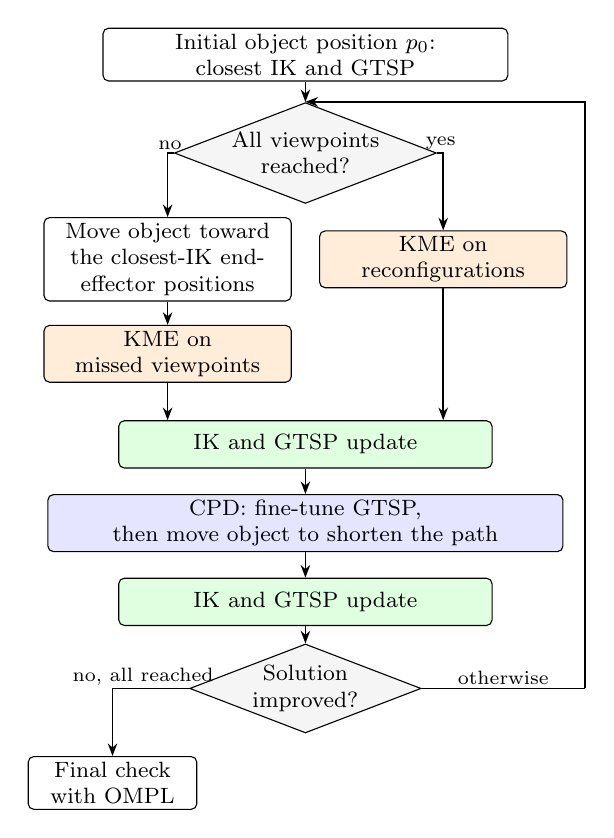
\begin{tikzpicture}[
  font=\footnotesize,
  box/.style={draw, rounded corners=2pt, align=center, minimum height=6mm, inner sep=2pt, text width=#1},
  box/.default=30mm,
  gtsp/.style={box=#1, fill=green!12},
  gtsp/.default=46mm,
  arr/.style={-{Stealth[length=1.6mm]}, semithick},
  lab/.style={font=\scriptsize, inner sep=1pt},
  dec/.style={draw, diamond, aspect=2.6, align=center, inner sep=0.3pt, fill=gray!8}
]
  \node[box=50mm] (init) at (0,0) {Initial object position $p_0$:\\closest IK and GTSP};
  \node[dec] (all) at (0,-1.25) {All viewpoints\\reached?};
  \node[box] (reach) at (-1.75,-2.6) {Move object toward the closest-IK end-effector positions};
  \node[box, fill=orange!15] (kmem) at (-1.75,-3.8) {KME on\\missed viewpoints};
  \node[box, fill=orange!15] (kmer) at (1.75,-2.6) {KME on\\reconfigurations};
  \node[gtsp] (g1) at (0,-4.95) {IK and GTSP update};
  \node[box=64mm, fill=blue!10] (rpd) at (0,-5.95) {CPD: fine-tune GTSP,\\then move object to shorten the path};
  \node[gtsp] (g2) at (0,-6.95) {IK and GTSP update};
  \node[dec] (any) at (0,-8.05) {Solution\\improved?};
  \node[box=20mm] (done) at (-2.45,-9.25) {Final check\\with OMPL};

  \coordinate (loopin) at (0,-0.6);
  \def\xr{3.55}
  \draw[arr] (init) -- (all);
  \draw[arr] (all.west) -| node[lab, above, pos=0.3] {no} (reach.north);
  \draw[arr] (all.east) -| node[lab, above, pos=0.3] {yes} (kmer.north);
  \draw[arr] (reach) -- (kmem);
  \draw[arr] (kmem.south) -- (kmem.south |- g1.north);
  \draw[arr] (kmer.south) -- (kmer.south |- g1.north);
  \draw[arr] (g1) -- (rpd);
  \draw[arr] (rpd) -- (g2);
  \draw[arr] (g2) -- (any);
  \draw[arr] (any.west) -| node[lab, above, pos=0.3] {no, all reached} (done.north);
  \draw[semithick] (any.east) -- node[lab, above] {otherwise} (\xr,-8.05);
  \draw[arr] (\xr,-8.05) -- (\xr,-0.6) -- (loopin);
\end{tikzpicture}

\caption{Pipeline overview. The method alternates between KME (orange) and CPD (blue). While viewpoints are missed, the object first moves toward the end-effector positions of their closest IK, and KME then expands the kinematic margins of the missed viewpoints; once all are reached, KME reduces the remaining reconfigurations. CPD fine-tunes the IK solutions and moves the object to shorten the coverage path. After each move step, the GTSP updates the coverage path (green). The loop repeats until the solution stops improving, and the final path is checked with OMPL.}
\label{fig:overview}
\end{figure}

\subsection{Overview}

We formulate the problem as a co-optimization of the object position and the coverage path, and solve it by alternating between two modules: KME, which reaches the missed viewpoints and reduces reconfigurations, and CPD, which shortens the coverage path. Since the IK solutions change along with the object movement, a GTSP replans the visiting order and IK solutions after each move step to update the coverage path.

\emph{KME.} At the current object position, this module first solves for the IK solution of each viewpoint. If a viewpoint does not have a valid IK solution, we compute its closest IK instead (Sec.~\ref{sec:closest}). The closest IK shows how near the end-effector can get to each missed viewpoint. The module then moves the object toward these closest-IK end-effector positions. After this move, some missed viewpoints become reachable, while others remain missed due to joint limits, singularities, or collisions. KME targets these remaining viewpoints: it moves the object along the gradient of their kinematic margins, computed through the robot Jacobian (Sec.~\ref{sec:kme}), while preserving the margins of the already reached viewpoints if possible. Subsequent moves can then bring more missed viewpoints within reach. Once every viewpoint is reached, KME treats each reconfiguration the same way, since it occurs where a margin shrinks to zero while the end-effector tracks the straight line between two viewpoints. After the KME move, the GTSP updates the visiting order and IK solutions at the new object position.

\emph{CPD.} This module unifies reach and path optimization: missed viewpoints are included in the coverage path through their closest IK, so path optimization is performed concurrently with viewpoint reaching. It proceeds in two steps. First, with the object fixed, it fine-tunes the GTSP solution obtained from KME. Using the robot arm's redundancy, the IK solution of each reached viewpoint is adjusted without moving the end-effector to shorten the coverage path. The IK solution of each missed viewpoint is re-solved starting from the IK solutions of its neighboring viewpoints along the path. For a 6-DOF robot arm, which has no redundancy, the adjustment of reached viewpoints is skipped. Second, CPD computes the gradient of the coverage path length $L$ in~\eqref{eq:length} with respect to the object position through the robot Jacobian, as in KME, and moves the object along it to shorten the path (Sec.~\ref{sec:evaluate}).

\begin{algorithm}[t]
\caption{Object placement and tour co-optimization}
\label{alg:descent}
\begin{algorithmic}[1]
\State $S \gets \textsc{Evaluate}(p_0)$, all IK solutions started from home
\While{time and iterations left}
  \If{some viewpoints are missed}
    \State move toward the misses; if rejected, KME
  \ElsIf{$R(S) > 0$}
    \State KME on the reconfigurations
  \EndIf
  \State arm-pose step: self-motion slides and GTSP reorder
  \State path step: move the object if $C$ drops
  \If{no step was accepted}
    \If{all viewpoints are reached} \textbf{break} \EndIf
    \State $\lambda \gets 10\lambda$; \textbf{break} if $\lambda > \lambda_{\max}$
  \EndIf
\EndWhile
\end{algorithmic}
\end{algorithm}

\subsection{Kinematic Margin}
\label{sec:margin}
The kinematic margin of a configuration $q$ at object position $p$ is formulated as
\begin{equation}
M(q, p) = \min\Big\{ \underbrace{\min_j \frac{\delta_j}{f_q}}_{\text{joint limit}},\; \underbrace{\frac{\sigma_{\min}(J)}{f_\sigma}}_{\text{singularity}},\; \underbrace{\min_k \frac{d_k}{f_d}}_{\text{clearance}} \Big\},
\label{eq:margin}
\end{equation}
Each term reflects one aspect of the kinematic margin and is divided by a normalization factor $f_q$, $f_\sigma$, or $f_d$ so that the terms are comparable. In the joint-limit term, $\delta_j = r_j(1 - |s_j|)$ is the distance of joint $j$ to its nearest limit, where $s_j = (q_j - c_j)/r_j \in (-1, 1)$ is the signed offset of the joint from the middle $c_j$ of its range, normalized by the half-range $r_j$. The singularity term is the smallest singular value of the tool Jacobian $J$, which vanishes at a singularity. In the clearance term, $d_k$ is the shortest distance between a robot link and the object, the environment, or another robot link. Hence, $M$ vanishes whenever the robot arm reaches any of these limits.

\subsection{Closest IK}
\label{sec:closest}
When there is no valid IK solution for a viewpoint, we use the Levenberg--Marquardt (LM) method to find its closest IK. It minimizes the pose error while keeping the joint-limit and clearance terms of the kinematic margin~\eqref{eq:margin} away from zero:
\begin{equation}
\begin{split}
E(q) = {}&\underbrace{\lVert e_p \rVert^2 + w_o \lVert e_o \rVert^2}_{\text{pose error}}
+ \underbrace{w_c \textstyle\sum_k \max(0, c - d_k)^2}_{\text{clearance margin}} \\
&+ \underbrace{w_l \textstyle\sum_j s_j^2 / (1 - s_j^2)}_{\text{joint-limit margin}},
\end{split}
\label{eq:closest}
\end{equation}
where $w_o$, $w_c$, and $w_l$ are weighting coefficients. The pose error term measures how far the end-effector is from the viewpoint, where $e_p$ and $e_o$ are the position and orientation errors. The clearance term penalizes any distance $d_k$ below a threshold $c$. The joint-limit term grows steeply as $|s_j|$ approaches 1, that is, as a joint approaches its limit. The singularity term is left out because the closest IK of an out-of-reach viewpoint is usually near a singularity, with the robot arm fully stretched toward it; penalizing it would pull the closest IK away from the viewpoint. The singularity issue is handled later by KME.

The LM solve starts from the viewpoint's previous IK and from three additional random starts. We keep the lowest-cost IK that is collision-free and whose end-effector has an unobstructed path to the viewpoint.

\subsection{Kinematic Margin Expansion}
\label{sec:kme}
KME moves the object along the gradients of the kinematic margin terms in~\eqref{eq:margin} w.r.t.\ the object position $p$. To compute these gradients, we first need the derivative of the IK $q_i$ of viewpoint $i$ w.r.t.\ the object position, which is given by
\begin{equation}
\frac{\partial q_i}{\partial p} = J_i^{+} \begin{bmatrix} I_3 \\ 0 \end{bmatrix} ,
\label{eq:follow}
\end{equation}
where $J_i = J(q_i)$ is the $6 \times n$ tool Jacobian and $I_3$ is the identity matrix. The damped pseudo-inverse $J_i^{+}$ is given by
\begin{equation}
J_i^{+} = J_i^{\top}(J_i J_i^{\top} + \mu^2 I)^{-1},
\label{eq:dpinv}
\end{equation}
where $\mu$ is a damping factor that prevents the joint motion from becoming excessively large near a singularity. At $q_i$, the gradients of the three kinematic margin terms are as follows.

\emph{Joint limit:}
\begin{equation}
\frac{d\delta_j}{dp} = -\operatorname{sgn}(s_j) \Big(\frac{\partial q_i}{\partial p}\Big)^{\!\top} e_j,
\label{eq:grad_joint}
\end{equation}
where $\operatorname{sgn}(s_j)$ is the sign of the offset $s_j$ and $e_j$ is the $j$-th unit vector.

\emph{Singularity:}
\begin{equation}
\frac{d\sigma_{\min}}{dp} = \Big(\frac{\partial q_i}{\partial p}\Big)^{\!\top} \nabla_q \sigma_{\min},
\label{eq:grad_sing}
\end{equation}
where $\nabla_q \sigma_{\min}$ is the gradient of the smallest singular value w.r.t.\ $q$.

\emph{Clearance:}
\begin{equation}
\frac{d\,d_k}{dp} = \Big(\frac{\partial q_i}{\partial p}\Big)^{\!\top} J_k^{\top} n_k - n_k,
\label{eq:grad_clear}
\end{equation}
where $n_k$ is the unit vector between the two closest points and $J_k$ is their relative Jacobian. The last term $-n_k$ accounts for the object itself moving, and appears only when $d_k$ is the distance between a robot link and the object.

For a missed viewpoint, $q_i$ is its closest IK. The move direction is a weighted sum of the gradients~\eqref{eq:grad_joint}--\eqref{eq:grad_clear} over all terms and all missed viewpoints:
\begin{equation}
d_{\text{KME}} = \sum_{i} \Big( \sum_j w^{\delta}_{ij} \frac{d\delta_j}{dp} + w^{\sigma}_{i} \frac{d\sigma_{\min}}{dp} + \sum_k w^{d}_{ik} \frac{d\,d_k}{dp} \Big),
\label{eq:room}
\end{equation}
where $i$ indexes the missed viewpoints, $j$ indexes the joints, and $k$ indexes the collision pairs. The weights of the joint-limit, singularity, and clearance terms are
\begin{equation}
\begin{aligned}
w^{\delta}_{ij} &= e^{-\delta_j / f_q},\\
w^{\sigma}_{i} &= e^{-\sigma_{\min} / f_\sigma},\\
w^{d}_{ik} &= e^{-d_k / f_d},
\end{aligned}
\label{eq:weights}
\end{equation}
where $\delta_j$, $\sigma_{\min}$, and $d_k$ are the joint-limit, singularity, and clearance terms at $q_i$, and $f_q$, $f_\sigma$, and $f_d$ are their normalization factors in~\eqref{eq:margin}. A term closer to zero receives a larger weight, so its gradient contributes more to the move direction. The direction $d_{\text{KME}}$ is then normalized to unit length.

We also calculate the gradient of each kinematic margin term $m$ close to zero at a reached viewpoint:
\begin{equation}
g = \frac{dm}{dp}\Big|_{q_i},
\label{eq:hurt}
\end{equation}
computed by~\eqref{eq:grad_joint}--\eqref{eq:grad_clear} at its IK $q_i$. Unlike in~\eqref{eq:room}, these gradients are not summed: for each one with $d_{\text{KME}}^\top g < 0$, the component of $d_{\text{KME}}$ that would decrease $m$ is removed:
\begin{equation}
d_{\text{KME}} \leftarrow d_{\text{KME}} - \frac{d_{\text{KME}}^\top g}{\|g\|^2}\, g.
\label{eq:project}
\end{equation}
This is repeated until no such term decreases, and the result is normalized. If too little of the direction remains, the original $d_{\text{KME}}$ is used. A move is accepted if it loses few reached viewpoints and reaches more or raises the smallest missed margin.

Once all viewpoints are reached, KME handles each reconfiguration the same way: the configuration where straight-line tracking stops takes the place of $q_i$ in~\eqref{eq:follow}--\eqref{eq:room}. A move is accepted if no viewpoint is lost and the number of reconfigurations drops, or stays the same while the smallest margin grows.

\subsection{Coverage-Path Placement Descent}
\label{sec:evaluate}
The descent combines the path length and the number of reconfigurations into one cost and adds two terms that guide it:
\begin{equation}
C = L + w_r R + w_j \sum_{i \in \mathcal{R}} \sum_{\ell} \max(0, b - d_{i\ell})^2 + \lambda \sum_{i \notin \mathcal{R}} g_i ,
\label{eq:cost}
\end{equation}
where $\mathcal{R}$ is the set of reached viewpoints, $d_{i\ell}$ the distance of joint $\ell$ of $q_i$ to its limit, $b$ a soft joint-room band, and $g_i$ the gap of missed viewpoint $V_i$, the distance from the end-effector at its closest IK to $V_i$. Motions whose straight joint move collides are charged their detour through the home configuration. We use $w_r = 2$, $w_j = 400$, $b = 0.05$~rad, and a gap weight $\lambda$ that starts at 100 per meter and grows when the descent stalls.

At a candidate position, each viewpoint's IK is solved by damped least squares started from its configuration at the previous position, so the robot arm follows the object and keeps its posture; if that fails, from a fallback configuration and then from up to 10 random starts. A viewpoint without an exact solution gets a closest configuration (Sec.~\ref{sec:closest}); closest configurations within 5~mm of the best gap are kept as alternatives. The visiting order and IK solutions are then replanned by the GTSP (Sec.~\ref{sec:gtsp}). Finally, the straight-line tracking of Sec.~\ref{sec:problem} runs along the path, missed viewpoints are re-solved from their neighbors' configurations, and the cost~\eqref{eq:cost} is computed. The reordered solution is kept if it reaches more viewpoints or costs less.

CPD first keeps the object fixed: a redundant robot arm can move each configuration along its self-motion without moving the tool. Each reached configuration is slid along
\begin{equation}
\Delta q_i = -\left(I - J_i^{+} J_i\right) \nabla_{q_i}\!\Big(L + w_j \sum_\ell \max(0, b - d_{i\ell})^2\Big),
\end{equation}
scaled so that the largest slide is 0.3~rad and halved on failure, and the position is evaluated (Sec.~\ref{sec:evaluate}) from the slid configurations. The step is kept if the cost drops by more than 0.05. For a 6-DOF robot arm the self-motion is empty and the step is skipped.

The object then moves along the gradient of the path length, which changes with the object through every IK solution, by~\eqref{eq:follow}:
\begin{equation}
d_{\text{path}} = -\sum_i \left(\frac{\partial q_i}{\partial p}\right)^{\!\top} \nabla_{q_i} L .
\end{equation}
It is combined with the analogous joint-limit direction after removing from each the component that opposes the other. The line search is as in the reach step. A move is accepted if the cost~\eqref{eq:cost} drops and, once all viewpoints are reached, it adds no reconfiguration, which would undo KME.

\emph{GTSP replanning.}\label{sec:gtsp} At every evaluated object position, the visiting order and IK solutions are replanned as a GTSP over IK candidates, starting from $q_0$ with the joint-space distance~\eqref{eq:length} as motion cost. The candidates of each viewpoint are its current IK solution and the IK solutions started from its neighbors along the path and from four fixed random configurations. The GTSP is solved by 2-opt, warm-started from the current order. Because reconfigurations are known only after tracking, each reconfiguring motion on the solved path is charged $w_r = 2$ and the GTSP is solved again, for two rounds.

\section{Experiments}
\subsection{Setup}
We use a 7-DOF UFactory xArm7 and a 6-DOF Universal Robots UR5e, each with a camera modeled as a cylinder on the flange \todo{dimensions per robot}. The objects are the Stanford bunny scaled to $8.0 \times 10.4 \times 10.3$~cm and the Stanford Armadillo scaled to 8~cm tall ($6.1 \times 6.7 \times 8.0$~cm)~\cite{stanford3dscan}. Viewpoints were generated once per object at 3~cm standoff with a 55$^\circ$ field of view, by greedy set cover up to 90\% of the visible area, which gives 33 viewpoints for the bunny and 19 for the Armadillo. A viewpoint counts as reached with safety margins of 1~cm from collision and 0.1~rad from the joint limits. The object may move within $x \in [0.2, 0.6]$, $y \in [-0.6, 0.6]$ and $z \in [-0.7, 0.7]$~m in the base frame, above the mounting surface. Each method starts from 32 positions, $x \in \{0.242, 0.342\}$, $y \in \{\pm 0.05, \pm 0.15\}$, $z \in \{0.107, 0.207, 0.307, 0.407\}$~m. A run succeeds if every viewpoint is reached and every motion plans. The GTSP is solved by a nearest-neighbor construction followed by up to five rounds of 2-opt on the visiting order alternated with IK re-selection for the fixed order, a standard GTSP local search~\cite{hu2008gtsp,gutin2010memetic}. The closest IK~\eqref{eq:closest} uses $c = 2$~cm, $w_o = 0.01$, $w_c = 1$ and $w_l = 10^{-4}$, with Levenberg--Marquardt steps of at most 0.1~rad. KME uses normalization factors $f$ of 0.05~rad, 0.02 and 1~cm for the joint-limit, singularity and collision margins. A term counts as close to zero below 6 for the missed viewpoints and below 2 for the reached ones, and a KME move may lose at most 10\% of the reached viewpoints. \todo{Time cap (600 s for all methods after the baseline reruns), CPU, seeds.}

When no step is accepted, the descent stops if every viewpoint is reached. Otherwise the gap weight $\lambda$ grows tenfold, up to $10^5$ per meter, and the descent continues. It also stops at the time budget or after 200 iterations. The result is then checked by planning every motion between consecutive viewpoints with OMPL: straight joint moves where they are collision-free, otherwise three 0.5~s planning attempts with the shortest path kept. A motion that fails is planned again with five 5~s attempts before it counts as failed. The reported path length is the planned joint path length, without the last wrist joint, which only spins the camera about its axis.

\subsection{Baselines}
\emph{SGD} follows Mayer and Althoff~\cite{mayer2026smart} (their Sec.~2.4) for the position: Adam steps along the averaged gradients of the closest-IK gaps, restarting near the best position so far until the budget runs out, and returning the first position that reaches every viewpoint with a plannable coverage path. \emph{CMA-ES}~\cite{hansen2016cmaes} searches the position as a black box (initial step 5~cm, default population size), scoring each candidate with our evaluation of Sec.~\ref{sec:evaluate} and ranking candidates by viewpoints reached, then gap, then cost~\eqref{eq:cost}. Both baselines are followed by our descent with the object frozen, so all three methods share the IK, the GTSP, the arm-pose step and the final check; only the placement differs. We do not compare with B*~\cite{bstar2025}, because it assumes a given visiting order and no reconfigurations, whereas here the order is free and every coverage path in Table~\ref{tab:results} still contains reconfigurations.

\subsection{Results}
% Seed 44, 32 starts per robot and object. Path length and reconfigurations: mean +- std over the starts where all three methods succeed (n).
% Success = all viewpoints reached and no failed edge.
% Ours: commit f0458c4, 600 s budget (bunny), 300 s (Armadillo) (noFe sweep). TODO: baselines ran at 300 s; replace after the baseline reruns.
\begin{table}[t]
\centering
\caption{Results over 32 start positions. Path length (rad) and reconfigurations: mean $\pm$ std over the $n$ starts where all methods succeed.}
\label{tab:results}
\setlength{\tabcolsep}{4pt}
\resizebox{\columnwidth}{!}{%
\begin{tabular}{llcccc}
\toprule
Object & Method & \multicolumn{2}{c}{xArm7} & \multicolumn{2}{c}{UR5e} \\
\midrule
 & & Success & Tour / Reconf. & Success & Tour / Reconf. \\
\midrule
\multirow{3}{*}{\shortstack[l]{Bunny\\($n$=31, 26)}}
 & SGD    & 32/32 & 42.2$\pm$7.7 / 6.4$\pm$2.0 & 29/32 & 53.8$\pm$12.1 / 8.2$\pm$3.0 \\
 & CMA-ES & 31/32 & 42.4$\pm$8.0 / 7.2$\pm$2.5 & 29/32 & 55.1$\pm$11.7 / 7.8$\pm$2.6 \\
 & Ours   & 32/32 & \textbf{38.5$\pm$5.8} / \textbf{5.3$\pm$2.2} & \textbf{32/32} & \textbf{38.8$\pm$6.4} / \textbf{4.3$\pm$1.3} \\
\midrule
\multirow{3}{*}{\shortstack[l]{Armadillo\\($n$=32, 32)}}
 & SGD    & 32/32 & 27.7$\pm$5.4 / 4.1$\pm$1.6 & 32/32 & 35.7$\pm$6.0 / 5.5$\pm$1.5 \\
 & CMA-ES & 32/32 & 24.0$\pm$4.7 / 4.0$\pm$1.7 & 32/32 & 35.0$\pm$6.1 / 5.3$\pm$1.5 \\
 & Ours   & 32/32 & \textbf{22.2$\pm$3.8} / \textbf{2.4$\pm$1.2} & 32/32 & \textbf{24.8$\pm$4.0} / \textbf{2.8$\pm$1.1} \\
\bottomrule
\end{tabular}}
\end{table}


Table~\ref{tab:results} reports the results. On the starts where all three methods succeed, our coverage paths are 15\% shorter than the baselines' on the bunny with the xArm7 and 27--28\% shorter with the UR5e; on the Armadillo they are 10--22\% (xArm7) and 30--31\% (UR5e) shorter. Reconfigurations drop by 38--53\% in every case. The advantage holds per start, not only on average: on the UR5e Armadillo, our coverage path is shorter than SGD's from 31 of the 32 starts, and has fewer reconfigurations from 29 of them. The gain is largest on the 6-DOF UR5e, which has no self-motion to absorb a poor placement, so the baselines' positions more often force posture changes that the GTSP cannot avoid. \todo{Paired statistics, e.g.\ Wilcoxon signed-rank, after the reruns.}

Our method succeeds from all 128 starts, while SGD and CMA-ES each fail from 3 of the 32 bunny starts on the UR5e, and CMA-ES from one on the xArm7. Our method converges in a median of 44~s and 98~s on the bunny (xArm7, UR5e) and 26~s and 50~s on the Armadillo; one of the 128 runs took longer than 300~s (330~s). \todo{Update with the 600 s baseline results.}

\begin{figure}[t]
\centering
\figplaceholder{Tour comparison from one start: ours vs.\ SGD, object position and tool path, reconfigurations marked.}{4cm}
\caption{\todo{caption}}
\label{fig:tour}
\end{figure}

\subsection{Ablation}
% Seed 44, 32 starts per robot and object; budget as the main runs (bunny 600 s, Armadillo 300 s, bunny with eggs 600 s). All variants rerun on the current code (full bunny: 28/32 on the UR5e vs 29/32 in tab:results, older code).
% w/o KME: co_room off; w/o CPD: co_tour_object_move off. Path and reconfigurations: mean +- std over the n starts where all three variants succeed.
% Runs: session f686a87f scratchpad/ablation (Armadillo full: session 417803c8 scratchpad/sweep/armadillo_seed44).
\begin{table}[t]
\centering
\caption{Ablation over 32 start positions. Path length (rad) and reconfigurations: mean $\pm$ std over the $n$ starts where all variants succeed.}
\label{tab:ablation}
\setlength{\tabcolsep}{4pt}
\resizebox{\columnwidth}{!}{%
\begin{tabular}{llcccc}
\toprule
Object & Variant & \multicolumn{2}{c}{xArm7} & \multicolumn{2}{c}{UR5e} \\
\midrule
 & & Success & Path / Reconf. & Success & Path / Reconf. \\
\midrule
\multirow{3}{*}{\shortstack[l]{Bunny\\($n$=29, 10)}}
 & Full    & 32/32 & \textbf{36.1$\pm$4.7} / \textbf{4.2$\pm$1.7} & 28/32 & \textbf{39.3$\pm$5.9} / \textbf{4.7$\pm$1.3} \\
 & w/o KME & 29/32 & 38.6$\pm$6.7 / 5.7$\pm$1.6 & 22/32 & 46.2$\pm$9.5 / 7.7$\pm$2.5 \\
 & w/o CPD & 32/32 & 37.2$\pm$5.6 / 5.0$\pm$1.8 & 15/32 & 50.1$\pm$6.5 / 5.8$\pm$1.1 \\
\midrule
\multirow{3}{*}{\shortstack[l]{Armadillo\\($n$=32, 25)}}
 & Full    & 32/32 & 22.1$\pm$3.3 / \textbf{2.3$\pm$1.2} & 31/32 & \textbf{24.9$\pm$3.9} / \textbf{2.8$\pm$1.2} \\
 & w/o KME & 32/32 & \textbf{21.9$\pm$3.6} / 2.9$\pm$1.4 & 26/32 & 25.0$\pm$3.8 / 3.6$\pm$1.2 \\
 & w/o CPD & 32/32 & 22.8$\pm$3.6 / 2.4$\pm$1.1 & 31/32 & 26.6$\pm$4.9 / 3.1$\pm$1.4 \\
\midrule
\multirow{3}{*}{\shortstack[l]{Bunny w/ eggs\\($n$=27, 30)}}
 & Full    & 32/32 & \textbf{46.6$\pm$6.9} / \textbf{5.3$\pm$2.3} & 32/32 & \textbf{45.6$\pm$7.1} / \textbf{3.6$\pm$1.3} \\
 & w/o KME & 27/32 & 49.1$\pm$8.5 / 6.7$\pm$2.9 & 30/32 & 46.1$\pm$7.3 / 5.1$\pm$1.9 \\
 & w/o CPD & 31/32 & 53.3$\pm$6.8 / 6.1$\pm$2.4 & 32/32 & 53.4$\pm$9.2 / 5.7$\pm$3.1 \\
\bottomrule
\end{tabular}}
\end{table}


We remove one module at a time, keeping every other parameter: \emph{w/o KME} turns off the margin expansion on both missed viewpoints and reconfigurations, and \emph{w/o CPD} lets the object move only for reach. Besides the bunny and the Armadillo, we add a bunny holding eggs with 65 viewpoints. Table~\ref{tab:ablation} reports the results from the same 32 starts. Without KME, 26 of the 192 runs fail, against 5 for the full method; 25 of them stop with viewpoints missed, where no reach step frees the blockers. On the starts where all variants succeed, it also leaves 26--64\% more reconfigurations in every case, since the reconfigurations no longer get room, while the path changes by $-1$ to $+18$\%. Without CPD, 19 runs fail, 17 of them on the bunny with the UR5e, which stop 1--4 viewpoints short. Its paths are longer in every case: by 14--27\% on the bunny with the UR5e and on the bunny with eggs, and by 3--7\% otherwise. KME thus mainly decides whether every viewpoint is reached and how many reconfigurations remain, and CPD decides the path length.

\subsection{Real-Robot Demonstration}
We executed the coverage paths optimized by our method for all three objects, the bunny, the Armadillo, and the bunny with eggs, on a real UR5e robot arm, with each object placed at its computed position. Each optimization started with the object midway between the end-effector at the home configuration and the ground. \todo{Figure of the execution.}

\section{Discussion and Limitations}
The method trades run time for path quality: it re-solves the IK and the path at every candidate position, and on the UR5e bunny a few starts needed several hundred seconds of reach and KME moves before the last viewpoints came in. Three UR5e bunny starts stopped with 29 of 33 viewpoints reached, where no move freed the remaining blockers. Only the object position is optimized, with its orientation fixed; the kinematic margin slopes extend directly to rotations. The viewpoints fix the camera's roll about its axis; leaving it free would add IK solutions and likely remove further reconfigurations. Finally, the method plans free motions between discrete tool poses; tasks that require the tool to stay in contact between poses need a motion model that follows the surface.

\section{Conclusion}
We presented a single-descent co-optimization of the object placement and the coverage path of a fixed-base manipulator. By moving the object to free the joint-limit, singularity and collision kinematic margins at the viewpoints that block reach and straight tool paths, and by re-solving the GTSP over IK candidates at every step, it yields shorter coverage paths with far fewer reconfigurations than placement baselines that share the same coverage path planner. Future work includes optimizing the object orientation, a free camera roll, and contact tasks.

\bibliographystyle{IEEEtran}
\bibliography{refs}

\end{document}
